
%% introduction

Finally, based on the absence of dominance relationship, we propose a
new class of portfolio strategy called \emph{Low Overhead Portfolio} (LOP),
which alternates between several depth-based tiebreaking methods.
Unlike the simple alternating open list proposed in LAMA planner \cite{richter2010lama},
it prevents the interaction between the queues and maintains the original
expansion order of each queue, allowing a clear theoretical analysis.
Also, it targets a single-heuristics, multi-tiebreaking scenario, unlike
the multi-heuristic scenario assumed in LAMA's alternating open list.
% 
LOP has several interesting characteristics:
First, the number of evaluations of nodes with $f<f*$ with LOP is exactly the same as
those with any single tiebreaking strategy.
Also, it has a theoretical guarantee that
the number of evaluations of nodes with $f=f*$ is at most $N$ times the \emph{minimum} 
of the evaluations required by $N$ strategies in the portfolio.
% 
%%% removed, we curretntly do not have much clue
% To put it simply, this portfolio does not need additional computation
% and we get a speedup for free (aside from the negligeble differences).
% Also, it is characteristic in that it works with a single heuristic function.
% We also empirically evaluates LOP.


\subsection{Low-Overhead Portfolios for Combining Tie-Breaking Strategies}

As noted above, it is unknown prior to the search where the goal node
exists in a plateau. However, the previous experiment showed that the
best depth-based second-level tiebreaking among \ld, \fd, \rd depends on
the domain characteristics and none of \ld, \fd, \rd dominated each
other.  Here, one natural idea is to use a portfolio approach which
combine these three.

The simplest possible portfolio approach would be a standard algorithm portfolio
which executes two completely independent \astar processes $A_1$ and $A_2$ in parallel, where $A_1$ uses tiebreaking strategey $S_1$ and $A_2$ uses tiebreaking strategy $S_2$, and CPU resources are allocated equally to $A_1$ and $A_2$.
The portolio would terminate when either $A_1$ or $A_2$ finds a goal state.
Let $T_1$ be the time that $A_1$ requires to solve instance $I$, and $T_2$ be the
time $A_2$ requires to solve instance $I$. Then, the total CPU time
required by the portfolio to solve instance $I$ is $2\times\min(A_1,A_2)$. This approach to combining multiple strategies is the standard algorithm portfolio proposed and analyzed in \cite{HubermanLH97,GomesS01}, and has also recently been called ``dovetailing'' and applied to combine multiple IDA* and \astar  \cite{ValenzanoSSBK10}. %TODO: remove the dovetailing reference after the paper is accepted -- the dovetailing authors were unaware of the HubermanLH97 paper...

On one hand, this simple portfoio approach has the advantage of mitigating worst-case risk -- as shown in \refig{plateau}, sometimes, the ratio between $T_1$ and $T_2$ is very large (e.g., $T_2 > 10\times T_1$) and choosing the wrong strategy has a very high penalty, so this portfolio strategy guarantees that the CPU usage is never more than twice that of using the faster strategy.
On the other hand, this simple portfolio will always require twice the
CPU time of the faster strategy.
%% removed, since LOP does not solve this problem
% Furthermore, the portfolio requires twice the RAM resources, which is a major disadvantage in memory-bound algorithms such as \astar.

We propose a new, \emph{Low-Overhead Portfolio} (LOP) implementation which can be used to implement a portfolio of tie-breaking strategies with significantly less overhead.
% 
Conceptually, a LOP for \astar is a portfolio composed of multiple
independently executing \astar where each \astar has completely separate
open/closed list, using a different tiebreaking strategy but sharing a
global cache for heuristic function values. Whenever a search engine
evaluates a state, it first checks the cache and reuses the result if
possible.  The current implementation is sequential -- each search
engine takes turns evaluating states. The algorithm finishes when some
engine finds the solution. Note that it takes turns \emph{evaluating}, not
\emph{expanding}, the states --- If we alternate the expansion, 
the node evaluation effort would not be evenly
distributed among \astar{}s, due to the difference in the number of
successor states of each node. There is a small pool for each queue
storing the nodes which are expanded
but not yet evaluated. Evaluation happens in turns, and if the pool is
exhausted, the expansion occurs as necessary in order to evaluate
more nodes.

Low-Overhead Portfolios offer some attractive tradeoffs,
particularly when runtimes are dominated by state evaluation, as is the case when searching with 
expensive heuristics such as LM-cut or recently proposed LP-based heuristics \cite{PommereningRHB14,ImaiF14}.

First, although the effort to insert/extract nodes from multiple
open/closed lists is doubled, these overheads are neglibigle when the
heuristic is expensive (see \refig{ffff}, left).

Second, although maintaining multiple open/closed lists requires additional memory,
when the heuristic is expensive enough, runtime becomes a bigger issue
than memory exhaustion  -- we show that with a 30 minute time limit, LOP
configurations do not exhaust memory more often than the other
configurations does (\refig{ffff}, right).

Third, node evaluation overheads for $f < f^*$ are eliminated due to the $h$-cache.
Recall that \astar always evaluates all states whose $f$ costs 
below $f^*$. Since the heuristic function $h$ and in turn $f=g+h$ are
the same among tiebreaking strategies, they evaluate the same set of
nodes with $f<f^*$. Unlike a standard portfolio implementation where 
nodes with $f<f^*$ would be evaluated multiple times, there is no evaluation overhead in a LOP
for nodes with $f<f^*$.
This is not
affected by the reopening caused by inconsitent heuristics either,
because the $h$-value is cached.

%% Third, since the search terminates when \emph{some} engine finds a
%% solution, and since the evaluation happens in turns, the search effort
%% within the final plateau is upper bounded by \emph{twice} the
%% \emph{minimum} of the search efforts required by each of \ld-\lifo or
%% \ld-\fifo engine alone.  Evaluating the same nodes in different engines
%% also reduces the effort to less than twice due to caching.  This is
%% desirable because, as we saw in the Results section, in some domains the
%% gap between the best and worst tiebreaking strategy can be more than 10
%% times (Openstacks, for example).  When there are $n$ engines, then this
%% increases to $n\times$ minimum amount of effort which would be spent by
%% each single engine alone.

Finally, in the worst case, the total number of nodes evaluated by a LOP is bounded by the number of nodes with $f \leq f^*$, which is the same as the worst-case behavior of \astar using the worst possible tie-breaking strategy.
This can occur  when all tiebreaking
strategies perform poorly  and they all evaluates the goal node in the
final iteration.

\subsubsection{Evaluating LOPs}

As we see in the previous section, the planner performance is greatly
affected by the tiebreaking criteria, especially when the search plateau
is huge, which is more often the case with the more practical,
cost-minimization domains.
% 
Also, the different depth-based tiebreakings are not dominating
each other and is unpredictably affected by the domain characteristics.
% 
Therefore, the LOP strategy should avoid the
worst-case scenario caused by bad tiebreaking, and quickly find the solution.

First, we show that the doubled cost of insertion and deletion by LOP is
negligeble.  We verified this by comparing the runtime of single \astar
with a LOP consisting of two same \astar, where all three \astar{}s
using the idential configuration ($[f,h,\fifo]$ with $h=$\lmcut). The
results in \refig{ffff} show that the extra cost of duplicated effort
is negligeble.

\begin{figure}[tb]
 \centering \relsize{-2}
 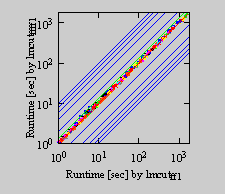
\includegraphics{tables/aaai16-30min/aaai16prelim3/time-nokey-lmcut_ff-lmcut_ffff.pdf}
 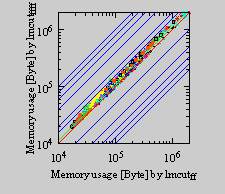
\includegraphics{tables/aaai16-30min/aaai16prelim3/mem-nokey-lmcut_ff-lmcut_ffff.pdf}
 \caption{Comparison of the runtimes (left) and memory usage (right) by
 single $[f,h,\fifo]$ and a LOP engine with 2 different instances of
 $[f,h,\fifo]$. Each line shows $\times 2,4,6\ldots$ boundary.
 The runtime gap was on average 1.03x and at most x1.29.
 The memeory usage gap was on average 1.14x and at most x1.56.
 We ignore the subsecond differences.}  \label{ffff}
 % this is from 30 min data. 9/7
\end{figure}

Next, we evaluated our LOP
strategy with selective combinations of two or three tiebreakings.
The configuration shown as ``lmcut m2'', ``lmcut m3'', ``mands m2'',
``lmcut m3'' are respectively the portfolio of
$[\ld,\fifo]$ + $[\rd,\lifo]$, $[\ld,\fifo]$ + $[\ld,\ro]$ + $[\rd,\lifo]$,
$[\ld,\fifo]$ + $[\rd,\ro]$, $[\ld,\fifo]$ + $[\rd,\ro]$ + $[\ld,\lifo]$. These
portfolios are selected by hand based on the previous results.
% LOP is able to avoid the accidental bias
Results in \reftbl{portfolio-coverage}
shows a significant improvements compared to the results by each search
engine alone.
% 
Also, \refig{portfolio-runtime} shows the number of evaluations of these
tiebreakings compared to each search engine alone.  It shows that
LOP acutally follows the expected behavior and the theoretical
bounds: the evaluation never exceeds twice/thirds of the single
search engine.

\begin{table}[tb]
 \centering \relsize{-2}
 \begin{tabular}{|c|c|c|c|}
\hline         
 Domain & \rotatebox[origin=l]{90}{${\mbox{lmcut}}_{\mbox{${\mbox{rd}}_{\mbox{random}}$}}$}   & \rotatebox[origin=l]{90}{${\mbox{lmcut}}_{\mbox{${\mbox{ld}}_{\mbox{random}}$}}$}   & \rotatebox[origin=l]{90}{${\mbox{lmcut}}_{\mbox{${\mbox{ldrd}}_{\mbox{random}}$}}$}    \\
\hline         
 sum(1104) &  \textbf{613} &  610 &  \textbf{613}  \\
\hline         
 {\relsize{-1}cybersec(19)} &  10 &  7 &  \textbf{11}  \\
 {\relsize{-1}gripper(20)} &  \textbf{7} &  \textbf{7} &  6 \\
\hline
 sum(380) &  184 &  \textbf{189} &  184  \\
\hline         
 {\relsize{-1}airport-fuel(20)} &  15 &  \textbf{16} &  \textbf{16}  \\
 {\relsize{-1}driverlog-fuel(20)} &  \textbf{9} &  8 &  8  \\
 {\relsize{-1}hiking-fuel(20)} &  \textbf{11} &  \textbf{11} &  10  \\
 {\relsize{-1}miconic-up(30)} &  \textbf{23} &  \textbf{23} &  22  \\
 {\relsize{-1}mprime-succumb(35)} &  22 &  \textbf{26} &  24  \\
 {\relsize{-1}tpp-fuel(30)} &  11 &  \textbf{12} &  11 \\
\hline
 sum(260) &  149 &  \textbf{150} &  147  \\
\hline         
 {\relsize{-1}elevators-up(20)} &  \textbf{11} &  \textbf{11} &  10  \\
 {\relsize{-1}freecell-move(20)} &  19 &  \textbf{20} &  \textbf{20}  \\
 {\relsize{-1}mystery-feast(20)} &  \textbf{9} &  \textbf{9} &  8  \\
 {\relsize{-1}pipesnt-pushstart(20)} &  11 &  11 &  \textbf{12}  \\
 {\relsize{-1}pipesworld-pushend(20)} &  \textbf{10} &  \textbf{10} &  9  \\
 {\relsize{-1}scanalyzer-analyze(20)} &  \textbf{11} &  9 &  10  \\
 {\relsize{-1}sokoban-pushgoal(20)} &  \textbf{20} &  19 &  19  \\
 {\relsize{-1}storage-lift(20)} &  5 &  \textbf{6} &  \textbf{6}  \\
 {\relsize{-1}woodworking-cut(20)} &  8 &  \textbf{10} &  8 \\
\hline
 total(1744) &  946 &  \textbf{949} &  944 \\
\hline
\end{tabular}

 \caption{Coverage results comparing some LOP combinations and the
 single strategies under the portfolio. The seeds are fixed to 1 in these instances.}
 \label{portfolio-coverage}
\end{table}

\todo{the evaluations are double-counted for LOP}

\begin{figure}[tb]
 \centering
 \relsize{-2}
 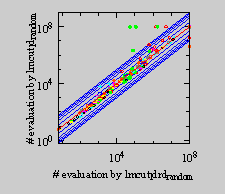
\includegraphics{tables/aaai16-multi-ldrd/zerocost/evaluated-nokey-lmcut_ldrd_random-lmcut_ld_random.pdf}
 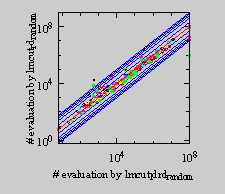
\includegraphics{tables/aaai16-multi-ldrd/zerocost/evaluated-nokey-lmcut_ldrd_random-lmcut_rd_random.pdf}
 \caption{Comparson of node evaluation between LOP $[\ld,\ro]$ +
 $[\rd,\ro]$ and the single strategy $[\ld,\ro]$ and $[\rd,\ro]$, on
 zerocost instances.}  \label{portfolio-runtime}
\end{figure}


%% related work

%% this will invoke a request from the reviewers to compare ours against it
%% * True, but people who know LAMA/FD are likely to demand some kind of comparison with alternating queues and preferred queues whether we mention  it or not.
%% Probably better to preemptively settle these questions rather than risking difficult questions during rebuttal.

Fast Downward/LAMA implement an \emph{alternation}
method \cite{Helmert2006} for OPEN list. It was originally used as a method for using
multiple heuristics in a planner.  There are multiple open lists, where there is a list for each heuristic, and states are
inserted into all lists according to the heuristic value for each
heuristic.  The major difference of alternation list to LOP is threefold:
First, LOP uses a single, expensive heuristic as the primary sorting
criteria ($f$-value), and it does not alternates between multiple
heuristics. Second, unlike alternation list alternates the
\emph{expansion}, LOP alternates the \emph{evaluation}.
Third, since the results of expansion in one list are inserted to all lists,
it changes the original insertion order in each queue.

Preferred operator queues are an extension of queue alternation, where in addition to the basic queue for each heuristic, there is a queue for states that are \emph{preferred} according to each heuristic \cite{richter2010lama}.
Although this was designed for non-admissible search in LAMA, preferred operators could, in principle, be applied to admissible search. 
Preferred operators are implemented by adding operator (state) preference computation to heuristic evaluator, and are therefore dependent on the heuristic function.
% Evidence: \cite{richter2010lama}, p.132 ``Operators that are deemed particularly useful in a given state are marked as preferred.   They are computed by the heuristic estimators along with the heuristic value of a state (see Sections 6 and 5).  
% More Evidence: \cite{richter2010lama}, p.150, last paragraph: ``We also generate preferred operators along with the landmark heuristic. An operator is preferred in a state if applying it achieves an acceptable landmark in the next step, i. e., a landmark whose pre-decessors have already been accepted.  If no acceptable landmark can be achieved within one step, the preferred operators are those which occur in a relaxed plan to a nearest acceptable landmark. A nearest landmark in the cost-unaware setting is one that is relaxed reachable with a
In contrast, the tie-breaking strategies investigated in this paper are implemented completely independently of the heuristic -- all of the tie-breaking stratgies in this paper can be applied to search using a blind heuristic.

%Lazy A* \cite{TolpinBSFK13} 
%TODO:  lazy A* vs LOP -- LazyA* combines multiple heuristics h1,h2 with low-overhead. However, if there is no dominance between h1,h2, behavior is different than h2; in contrast, LOP guarantees conservative behavior. % no, never mind, too different..
